% Set up the document
\documentclass{article}

% Page size
\usepackage[
    letterpaper,]{geometry}

% Lines between paragraphs
\setlength{\parskip}{\baselineskip}
\setlength{\parindent}{0pt}

% Math
\usepackage{mathtools}
\usepackage{amssymb}

\DeclareMathOperator\supp{supp}

% Links
\usepackage{hyperref}

% Page numbers at top right
\usepackage{fancyhdr}
\pagestyle{fancy}
\fancyhf{}
\fancyhead[R]{\thepage}
\renewcommand\headrulewidth{0pt}

% Graphics
\usepackage{float}
\usepackage{graphicx}
\graphicspath{ {./plots/img/} }

\begin{document}

\textbf{MATH 418 Homework 2} \\
\textbf{Matt Wiens \#301294492} \\
\textbf{2019-09-23}

1. [4.9.4] Suppose $u(x, y)$ satisfies
%
\begin{equation*}
    u_x+y^2 u_y = 0
\end{equation*}
%
Suppose further that
%
\begin{align*}
    u(3, 2) &= 7 \\
    u(4, 2) &= -6 \\
    u(8, 1) &= -2 \\
    u(6, -1) &= 3 \\
    u(6, -2) &= 0 \\
    u(10, 7) &= 8 \\
    u(15, -4) &= 10
\end{align*}
%
What are the values of $u\left(\frac{5}{2}, \frac{1}{2}\right)$ and
$u\left(8,-\frac{2}{5}\right)$? Can you find the value of
$u\left(\frac{9}{2},1\right)$? Explain your reasoning.

\textbf{Solution}

soln here

\vspace{5mm}

[4.9.26] Use the Method of Characteristics to solve
%
\begin{equation*}
    (y + u) u_x + y u_y = x - y, \quad u(x, 1) = 1 + x
\end{equation*}
%
\textbf{Solution}

Using the Method of Characteristics we set up the following system of
equations:
%
\begin{equation*}
    \begin{dcases}
        \frac{d x}{d s} = y + U \\
        \frac{d y}{d s} = y \\
        \frac{d U}{d s} = x - y \\
        \left( x(0), y(0), U(0)\right) = \left( x_0, 1, 1 + x_0 \right)
    \end{dcases}
\end{equation*}
%
We first solve for $y(s)$:
%
\begin{equation*}
    y(s) = \exp(s)
\end{equation*}
%
Which leaves us with
%
\begin{equation*}
    \begin{dcases}
        \frac{d x}{d s} = e^s + U \\
        \frac{d U}{d s} = x - e^s \\
        \left( x(0), U(0)\right) = \left( x_0, 1 + x_0 \right)
    \end{dcases}
\end{equation*}
%
Taking a derivative in the equation for $x^{\prime}(s)$ we have, for
some constants $A, B \in \mathbb{R}$,
%
\begin{align*}
    &x^{\prime \prime} = e^s + U^{\prime} \\
    &\iff x^{\prime \prime} = e^s + \left(x - e^s\right) \\
    &\iff x^{\prime \prime} = x \\
    &\iff x(s) = A \exp(s) + B \exp(-s)
\end{align*}
%
Now we solve for $U(s)$ as follows:
%
\begin{align*}
    &u^{\prime}(s) = A \exp(s) + B \exp(-s) - \exp(s) \\
    &\Rightarrow u(s) = A \exp(s) - B \exp(-s) - \exp(s)
\end{align*}
%
To solve for $A$ and $B$ we use our initial conditions, which give us
the system
%
\begin{equation*}
    \begin{dcases}
        A + B = x_0 \\
        A - B - 1 = 1 + x_0
    \end{dcases}
\end{equation*}
%
which has solutions
%
\begin{align*}
    A &= 1 + x_0 \\
    B &= -1
\end{align*}
%
To summarize what we have so far, we have
%
\begin{equation*}
    \begin{dcases}
        x(s) = (1 + x_0) \exp(s) - \exp(-s) \\
        y(s) = \exp(s) \\
        U(S) = (1 + x_0) \exp(s) + \exp(-s) - \exp(s)
    \end{dcases}
\end{equation*}
%
We can solve easily for $s$ in terms of $y$:
%
\begin{equation*}
    s = \log y
\end{equation*}
%
Substituting this into the equation for $x$, we have
%
\begin{equation*}
    x = (1 + x_0) y - y^{-1}
\end{equation*}
%
which, when solving for $x_0$, gives
%
\begin{equation*}
    x_0 = x y^{-1} + y^{-2} - 1
\end{equation*}
%
Now we can solve for $u(x, y)$ as follows:
%
\begin{align*}
    u(x, y) &= U(s(x, y), x_0(x, y)) \\
            &= \left[1 + \left(x y^{-1} + y^{-2} - 1\right)\right] y - y + y^{-1} \\
            &= \frac{x y - y^2 + 2}{y}
\end{align*}

\newpage

2. Suppose $u$ is a solution to the equation
%
\begin{equation*}
    u_t + u u_x = 0, \quad u(0, x) = h(x)
\end{equation*}
%
(a) Let $h$ be the function
%
\begin{equation*}
    h(x) =
        \begin{cases}
            \frac{1}{2}, & x < -2 \\
            -\frac{1}{2}, & x > 2 \\
            -\frac{1}{4} x, & x \in [-2, 2]
        \end{cases}
\end{equation*}
%
Sketch the solution $u(t, x)$ at $t = 1, 2, 3$ in the $(x, u)$-plane.
Find their precise formulas. Can you find the first time that
characteristics start to collide?

\textbf{Solution}

Using the Method of Characteristics we set up the following system of
equations:
%
\begin{equation*}
    \begin{dcases}
        \frac{d t}{d s} = 1 \\
        \frac{d x}{d s} = U \\
        \frac{d U}{d s} = 0 \\
        \left( t(0), x(0), U(0)\right) = \left( 0, x_ 0, h(x_0) \right)
    \end{dcases}
\end{equation*}
%
We can easily solve for $t$ and $U$ to obtain
%
\begin{align*}
    t(s) &= s \\
    U(s) &= h(x_0)
\end{align*}
%
which lets us solve for $x$ to obtain
%
\begin{equation*}
    x(s) = h(x_0) s + x_0
\end{equation*}

Now, in terms of $t$ we have
%
\begin{align*}
    x(t) &=
        \begin{cases}
            \frac{1}{2} t + x_0, & x_0 < -2 \\
            -\frac{1}{2} t + x_0, & x_0 > 2 \\
            -\frac{1}{4} x_0 t + x_0, & x_0 \in [-2, 2]
        \end{cases}
    \\
    U(t) &=
        \begin{cases}
            \frac{1}{2}, & x_0 < -2 \\
            -\frac{1}{2}, & x_0 > 2 \\
            -\frac{1}{4} x_0, & x_0 \in [-2, 2]
        \end{cases}
\end{align*}
%
Plots of the solution are shown below:
%
\begin{figure}[H]
    \centering
    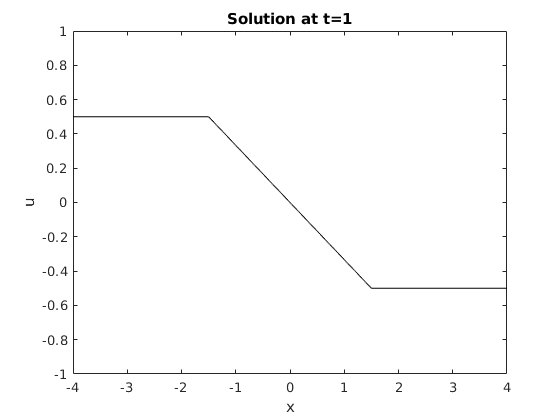
\includegraphics[width=12cm]{q2pa-1}
\end{figure}
%
\begin{figure}[H]
    \centering
    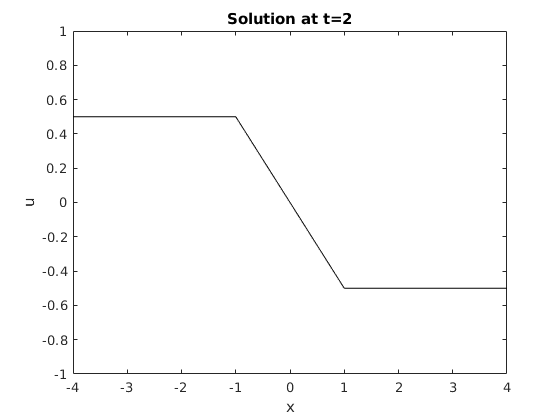
\includegraphics[width=12cm]{q2pa-2}
\end{figure}
%
\begin{figure}[H]
    \centering
    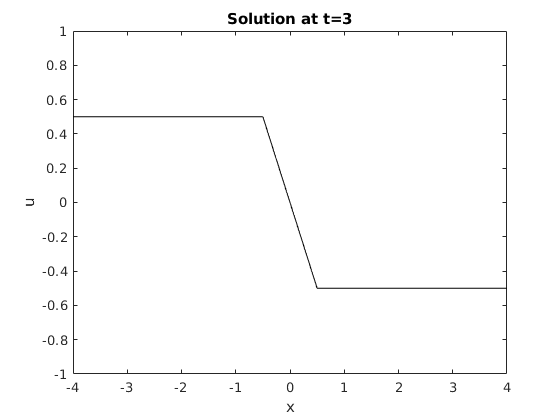
\includegraphics[width=12cm]{q2pa-3}
\end{figure}
%
From the plots it appears that the characteristics will collide at $x =
0$. We can solve for the exact time $t_c$ after which this occurs,
identifying this is the time immediately after which the left-most
characteristic reaches $x = 0$ (this is also the time after which the
right-most characteristic reaches $x = 0$):
%
\begin{align*}
    &\frac{1}{2} t_c - 2 = 0 \\
    &\Rightarrow t_c = 4
\end{align*}

\vspace{5mm}

(b) Sketch the solution $u(t, x)$ at $t = 1, 2, 3$ in $(x, u)$-plane and
find the precise formulas if we change the definition of $h$ into
%
\begin{equation*}
    h(x) =
        \begin{cases}
            -\frac{1}{2}, & x < -2 \\
            \frac{1}{2}, & x > 2 \\
            \frac{1}{4} x, & x \in [-2, 2]
        \end{cases}
\end{equation*}
%
In this case will the characteristics collide?

\textbf{Solution}

With this new definition for $h$ we follow the same steps as in part
(a), and then substituting in the new $h$ we have
%
\begin{align*}
    x(t) &=
        \begin{cases}
            -\frac{1}{2} t + x_0, & x_0 < -2 \\
            \frac{1}{2} t + x_0, & x_0 > 2 \\
            \frac{1}{4} x_0 t + x_0, & x_0 \in [-2, 2]
        \end{cases}
    \\
    U(t) &=
        \begin{cases}
            -\frac{1}{2}, & x_0 < -2 \\
            \frac{1}{2}, & x_0 > 2 \\
            \frac{1}{4} x_0, & x_0 \in [-2, 2]
        \end{cases}
\end{align*}
%
Plots of the solution are shown below:
%
\begin{figure}[H]
    \centering
    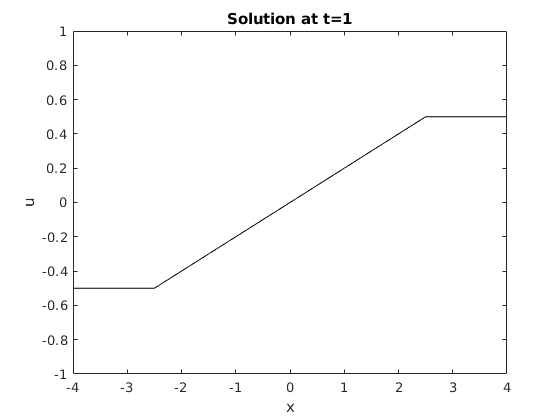
\includegraphics[width=12cm]{q2pb-1}
\end{figure}
%
\begin{figure}[H]
    \centering
    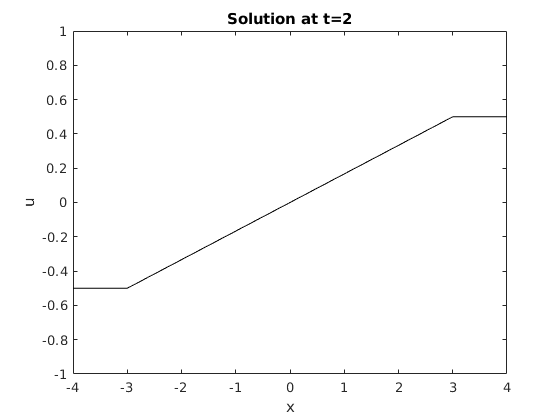
\includegraphics[width=12cm]{q2pb-2}
\end{figure}
%
\begin{figure}[H]
    \centering
    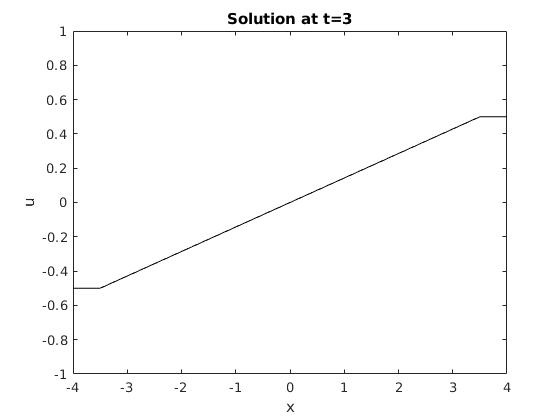
\includegraphics[width=12cm]{q2pb-3}
\end{figure}
%
We can see in this case that the characteristics will \textit{not}
colide.

\newpage

3. (a) Suppose $f, g$ are continuous on $[-10, 10]$ and
%
\begin{equation*}
    \int_{-10}^{10} f(x) h(x) \mathrm{d} x = \int_{-10}^{10} g(x) h(x)\mathrm{d} x
    \quad \text { for any } h \text { integrable on } [-10, 10]
\end{equation*}
%
Show that $f(x) = g(x)$ for all $x \in [-10, 10]$.

\textbf{Solution}

The proof that follows closely mirrors the fundamental lemma of the
calculus of variations:

Suppose the conditions above hold. Then, clearly
%
\begin{equation}
    \int_{-10}^{10} \left(f(x) - g(x)\right) h(x) \mathrm{d} x = 0
    \quad \text { for any } h \text { integrable on } [-10, 10]
    \label{eq:q3pa}
\end{equation}
%
For convenience, let $M(x) = f(x) - g(x)$. Note that $M(x)$ is also
continuous on $[-10, 10]$. Suppose that $M(x)$ is either positive (or
negative) at some point in $[-10, 10]$. Since $M(x)$ is continuous, it
must be positive (or negative) in an interval $[x_1, x_2] \in [-10, 10]$.

Consider the integrable function $h$ defined as
%
\begin{equation*}
    h(x) =
        \begin{dcases}
            (x - x_1)^2 (x - x_2)^2, & x \in [x_1, x_2] \\
            0, & x \not\in [x_1, x_2]
        \end{dcases}
\end{equation*}
%
Then
%
\begin{align*}
    \int_{-10}^{10} M(x) h(x) \mathrm{d} x
        &= \int_{x_1}^{x_2} M(x) (x - x_1)^2 (x - x_2)^2 \mathrm{d} x \\
        &\neq 0
\end{align*}
%
But this contradicts \eqref{eq:q3pa}. Hence
%
\begin{align*}
    &M(x) = 0, \quad x \in [-10, 10] \\
    &\Rightarrow f(x) - g(x) = 0, \quad x \in [-10, 10] \\
    &\Rightarrow f(x) = g(x), \quad x \in [-10, 10]
\end{align*}

\vspace{5mm}

(b) Show that if $f \in C^{1}[a, b]$ with $a, b \in \mathbb{R}$, then
$f$ must be uniformly continuous on $[a, b]$.

\textbf{Solution}

Suppose $f \in C^1[a, b]$. Then there exists $M \in \mathbb{R}$ such
that $|f(x)| < M$ for all $x \in [a, b]$.

Fix any $\epsilon > 0$ and consider any $x, y \in [a, b]$. Then the mean
value theorem tells us that there exists $c \in [x, y]$ such that
%
\begin{equation*}
    f(y) - f(x) = f^\prime(c) (y - x)
\end{equation*}
%
Taking the absolute value of both sides we have
%
\begin{align*}
    &|f(y) - f(x)| = |f^\prime(c)| |y - x| \\
    &\iff |f(x) - f(y)| = |f^\prime(c)| |x - y| \\
    &\iff |f(x) - f(y)| < M |x - y| \\
\end{align*}
%
Hence if we take $\delta = \frac{\epsilon}{M}$ then for all $x, y \in [a, b]$
%
\begin{equation*}
    |x - y| < \delta
    \Rightarrow |f(x) - f(y)| < M |x - y| < M \frac{\epsilon}{M} = \epsilon
\end{equation*}
%
and hence f is uniformly continuous on $[a, b]$.

\vspace{5mm}

(c) Give a counterexample where $f_n \to f$ pointwise on
$\mathbb{R}$ but not uniformly.

\textbf{Solution}

A simple counterexample is a sequence of ``spike'' functions with
``height'' $1$:
%
\begin{equation*}
    f_n(x) =
        \begin{cases}
            n x, & 0 \leq x < \frac{1}{n} \\
            2 - n x & \frac{1}{n} \leq x < \frac{2}{n} \\
            0 & \frac{2}{N} \leq x
        \end{cases}
\end{equation*}
%
If we let $f: x \mapsto 0$, then for any $x \in \mathbb{R}$
%
\begin{equation*}
    \lim_{n \to \infty} f_n(x) = 0 = f(x)
\end{equation*}
%
and hence $f_n \to f$ in the pointwise sense.

However, for any $n \in \mathbb{N}$,
%
\begin{align*}
    \sup_{x \in \mathbb{R}} |f_n(x) - f(x)|
        &= \sup_{x \in \mathbb{R}} |f_n(x)| \\
        &= 1
\end{align*}
%
so $f_n \not\to f$ uniformly.

\newpage

4. (a) Show that if $f : \mathbb{R}^{d} \rightarrow \mathbb{R}$,
$f \in C^k(\mathbb{R}^d)$, then its distributional derivatives up to
order $k$ are equal to its classical derivatives up to order $k$.

\textbf{Solution}

Let $F$ be the distribution corresponding to a
function $f : \mathbb{R}^{d} \rightarrow \mathbb{R}$, $f \in
C^k(\mathbb{R}^d)$. Following the notation in lectures let $D_x^\alpha$
denote a specific $n$-th order derivative. For this problem, we take $n
\leq k$; i.e, $|\alpha| = n \leq k$. We want to show that for any such
$\alpha$, $D_x^\alpha F$ is equal to the distribution $G$ corresponding
to $D_x^\alpha f$.

We proceed by induction. For the case where $k = 1$ we want to show that
$\partial_{x_i}F = G$ where $G$ is the distribution corresponding to
$\partial_{x_i} f$. Let $\phi \in \mathcal{D}$. Then for some open and
bounded $\Omega \subset \mathbb{R}^d$, $\supp \phi \subset \Omega$. Let
$\Gamma = \partial \Omega$. Then, using the fact that $\phi$ vanishes on
$\Gamma$, we have
%
\begin{align*}
    \langle G, \phi \rangle
        &\equiv \int_{\mathbb{R}^d} \left[\partial_{x_i} f(x)\right] \phi(x) \mathrm{d} x \\
        &= \int_{\Omega} \left[\partial_{x_i} f\right] \phi \,\mathrm{d} \Omega \\
        &= \int_{\Gamma} f \phi \,\mathbf{e_i} \cdot \mathbf{\hat{n}} \,\mathrm{d} \Gamma
            - \int_{\Omega} f \left[ \partial_{x_i} \phi \right] \mathrm{d} \Omega \\
        &= - \int_{\Omega} f \left[ \partial_{x_i} \phi \right] \mathrm{d} \Omega \\
        &= - \int_{\mathbb{R}^d} f(x) \left[ \partial_{x_i} \phi(x) \right] \mathrm{d} x \\
        &\equiv \langle \partial_{x_i} F, \phi \rangle
\end{align*}
%
Thus $\partial_{x_i} F = G$.

Now suppose that for $k \leq m$, for any multi-index $\alpha$ with
$|\alpha| \leq k$, $D_x^\alpha F$ is equal to the distribution $G$
corresponding to $D_x^\alpha f$.

Let $n \leq m$, then consider any $(n + 1)$-th order derivative
$\partial_{x_i} D_x^\alpha$, where $|\alpha| <= n$. Letting $G$ be the
distribution corresponding to $\partial_{x_i} D_x^\alpha f$, we want to
show that $\partial_{x_i} D_x^\alpha F = G$.

Let $\phi \in \mathcal{D}$. For some open and bounded
$\Omega \subset \mathbb{R}^d$, $\supp \phi \subset \Omega$. Let
$\Gamma = \partial \Omega$. Let $H$ be the distribution
corresponding to $D_x^\alpha f$. Note that by hypothesis we have
%
\begin{equation*}
    H = D_x^\alpha F
\end{equation*}
%
Now,
%
\begin{align*}
    \langle G, \phi \rangle
        &\equiv \int_{\mathbb{R}^d} \left[\partial_{x_i} D_x^\alpha f(x)\right] \phi(x) \mathrm{d} x \\
        &= \int_{\Omega} \left[\partial_{x_i} D_x^\alpha f\right] \phi \,\mathrm{d} \Omega \\
        &= \int_{\Gamma} \left[D_x^\alpha f\right] \phi \,\mathbf{e_i} \cdot \mathbf{\hat{n}} \,\mathrm{d} \Gamma
            - \int_{\Omega} \left[D_x^\alpha f\right] \left[ \partial_{x_i} \phi \right] \mathrm{d} \Omega \\
        &= - \int_{\Omega} \left[D_x^\alpha f\right] \left[ \partial_{x_i} \phi \right] \mathrm{d} \Omega \\
        &= - \int_{\mathbb{R}^d} \left[D_x^\alpha f(x)\right] \left[ \partial_{x_i} \phi(x) \right] \mathrm{d} x \\
        &\equiv \langle \partial_{x_i} H, \phi \rangle \\
        &= \langle \partial_{x_i} D_x^\alpha F, \phi \rangle
\end{align*}
%
and hence $\partial_{x_i} D_x^\alpha F = G$, which completes the induction.

\vspace{5mm}

(b) Use the definition of the distributional derivative to find the
first-order derivative (in the distributional sense) of the function
%
\begin{equation*}
    h(x) =
        \begin{cases}
            0, & x < -2 \\
            2, & -2 \leq x \leq -1 \\
            0, & -1 < x < 1 \\
            1, & 1 \leq x \leq 2 \\
            0, & x > 2 \\
        \end{cases}
\end{equation*}
%
\textbf{Solution}

For the sake of clarity, let $H$ be the distribution corresponding to
$h$. Then for any $\phi \in \mathcal{D}$ we have
%
\begin{align*}
    \langle H^\prime, \phi \rangle
        &\equiv \langle H, \phi^\prime \rangle \\
        &= \int_{- \infty}^{\infty} h(x) \phi^\prime(x) \mathrm{d} x \\
        &= \int_{-2}^{-1} 2 \phi^\prime(x) \mathrm{d} x
            + \int_{1}^{2} \phi^\prime(x) \mathrm{d} x \\
        &= 2 \left( \phi(-1) - \phi(-2) \right) + \left( \phi(2) - \phi(1) \right) \\
        &= 2 \phi(-1) + \phi(2) - 2 \phi(-2) - \phi(1)
\end{align*}
%
Hence we identify
%
\begin{equation*}
    H^\prime = 2 \delta_{-1} + \delta_2 - 2 \delta_{-2} - \delta_1
\end{equation*}

\vspace{5mm}

(c) Suppose $f(x) = |x|$ on $\mathbb{R}$. Find $f^{\prime \prime}$
directly by using the definition of the second-order distributional
derivative. Then find $f^{\prime \prime}$ by treating it as the
first-order distributional derivative of $f^{\prime}$ (which is the
first-order distributional derivative of $f)$. Do they agree as
distributions?

\textbf{Solution}

Let $F$ be the distribution corresponding to $f$. We can find $F^\prime$
as follows:

Let $\phi \in \mathcal{D}$. Then, for some $l \in \mathbb{R}$, $\supp
\phi \subseteq [-l, l]$. Thus we have
%
\begin{align*}
    \langle F^\prime, \phi \rangle
        &\equiv \langle F, \phi^\prime \rangle \\
        &= \int_{- \infty}^{\infty} f(x) \phi^\prime(x) \mathrm{d} x \\
        &= \underbrace{\int_{0}^{l} x \phi^\prime(x) \mathrm{d} x}_{I_1}
            - \underbrace{\int_{-l}^{0} x \phi^\prime(x) \mathrm{d} x}_{I_2} \\
        &= I_1 - I_2
\end{align*}
%
with (using integration by parts)
%
\begin{align*}
    I_1 &= \int_{0}^{l} x \phi^\prime(x) \mathrm{d} x \\
        &= \big[ x \phi(x) \big]_{0}^{l} - \int_{0}^{l} \phi(x) \mathrm{d} x \\
        &= - \int_{0}^{l} \phi(x) \mathrm{d} x \\
        &= - \int_{0}^{\infty} \phi(x) \mathrm{d} x
\end{align*}
%
By similar calculation we have
%
\begin{equation*}
    I_2 = - \int_{- \infty}^{0} \phi(x) \mathrm{d} x
\end{equation*}
%
and hence
%
\begin{align*}
    \langle F^\prime, \phi \rangle
        &= I_1 - I_2 \\
        &= \int_{- \infty}^{0} \phi(x) \mathrm{d} x - \int_{0}^{\infty} \phi(x) \mathrm{d} x \\
        &= \int_{- \infty}^{\infty} g(x) \phi(x) \mathrm{d} x
\end{align*}
%
where
%
\begin{equation*}
    g(x) =
        \begin{cases}
            1, & x \leq 0 \\
            -1, & x > 0
        \end{cases}
\end{equation*}
%
for any $\phi \in \mathcal{D}$ Hence $F^\prime = G$ where $G$ is the
distribution corresponding to $g$.

Now, taking the first-order distributional derivative of $F^\prime$,
again let $\phi \in \mathcal{D}$ with $\supp \phi \subseteq [-l, l]$ for
some $l \in \mathbb{R}$. Then we have
%
\begin{align*}
    \langle F^{\prime \prime}, \phi \rangle
        &= \langle G^\prime, \phi \rangle \\
        &\equiv \langle G, \phi^\prime \rangle \\
        &= \int_{- \infty}^{\infty} g(x) \phi^\prime(x) \mathrm{d} x \\
        &= - \int_{0}^{l} \phi^\prime(x) \mathrm{d} x
            + \int_{-l}^{0} \phi^\prime(x) \mathrm{d} x \\
        &= - \left( \phi(l) - \phi(0) \right) + \left( \phi(0) - \phi(-l) \right) \\
        &= 2 \phi(0) \\
\end{align*}
%
and hence we identify
%
\begin{equation*}
    F^{\prime \prime} = 2 \delta_0
\end{equation*}
%
We can also find $F^{\prime \prime}$ by using the definition of the
second-order distributional derivative:

Let $\phi \in \mathcal{D}$ with $\supp \phi \subseteq [-l, l]$ for some
$l \in \mathbb{R}$. Then we have
%
\begin{align*}
    \langle F^{\prime \prime}, \phi \rangle
        &\equiv \langle F, \phi^{\prime \prime} \rangle \\
        &= \int_{- \infty}^{\infty} f(x) \phi^{\prime \prime}(x) \mathrm{d} x \\
        &= \underbrace{\int_{0}^{l} x \phi^{\prime \prime}(x) \mathrm{d} x}_{I_3}
            - \underbrace{\int_{-l}^{0} x \phi^{\prime \prime}(x) \mathrm{d} x}_{I_4} \\
        &= I_3 - I_4
\end{align*}
%
where we calculate
%
\begin{align*}
    I_3 &= \int_{0}^{l} x \phi^{\prime(x) \prime} \mathrm{d} x \\
        &= \big[ x \phi^\prime(x) \big]_{0}^{l} - \int_{0}^{l} \phi^\prime(x) \mathrm{d} x \\
        &= \phi(0)
\end{align*}
%
and similarly
%
\begin{equation*}
    I_4 = - \phi(0)
\end{equation*}
%
Hence
%
\begin{align*}
    \langle F^{\prime \prime}, \phi \rangle
        &= I_3 - I_4 \\
        &= (\phi(0)) - (- \phi(0)) \\
        &= 2 \phi(0)
\end{align*}
%
and hence we, again, identify
%
\begin{equation*}
    F^{\prime \prime} = 2 \delta_0
\end{equation*}
%
which agrees with our previous calculation.

\end{document}
